\section{NASA-TLX Cognitive Load}
In this section, we present the results of NASA-TLX cognitive load across experiment groups using descriptive statistics, a Bayesian model, and qualitative findings from post-survey interviews to address how the number of options in Quadratic Surveys (QS) (\textbf{RQ1}) and the interface design (\textbf{RQ2a}) impact cognitive load.

For the qualitative analysis, the first author conducts an inductive thematic analysis~\cite{olsonWaysKnowingHCI2014} after transcribing the interviews. Snippets are initially coded based on the research questions and topics of interest, with similar codes merged to form overarching themes. When differences emerges across experiment conditions and hypotheses are identified, a deductive coding process is applied to refine and validate the findings.

For quantitative analysis, we employ a Bayesian approach to enhance transparency and provide a probabilistic interpretation of results, moving beyond binary significance thresholds~\cite{kay2016researcher}. Bayesian methods allow for the interpretation of posterior distributions and are well-suited for both large and small sample sizes due to the use of priors based on maximum entropy distributions, which ensure conservative and robust inferences~\cite{mcelreath2018statistical}.

\begin{figure}[htbp]
    \centering
    \adjustbox{valign=t}{ % Adjust first subfigure for top alignment
        \begin{subfigure}{0.47\textwidth}
            \centering
            \adjustbox{valign=t}{
                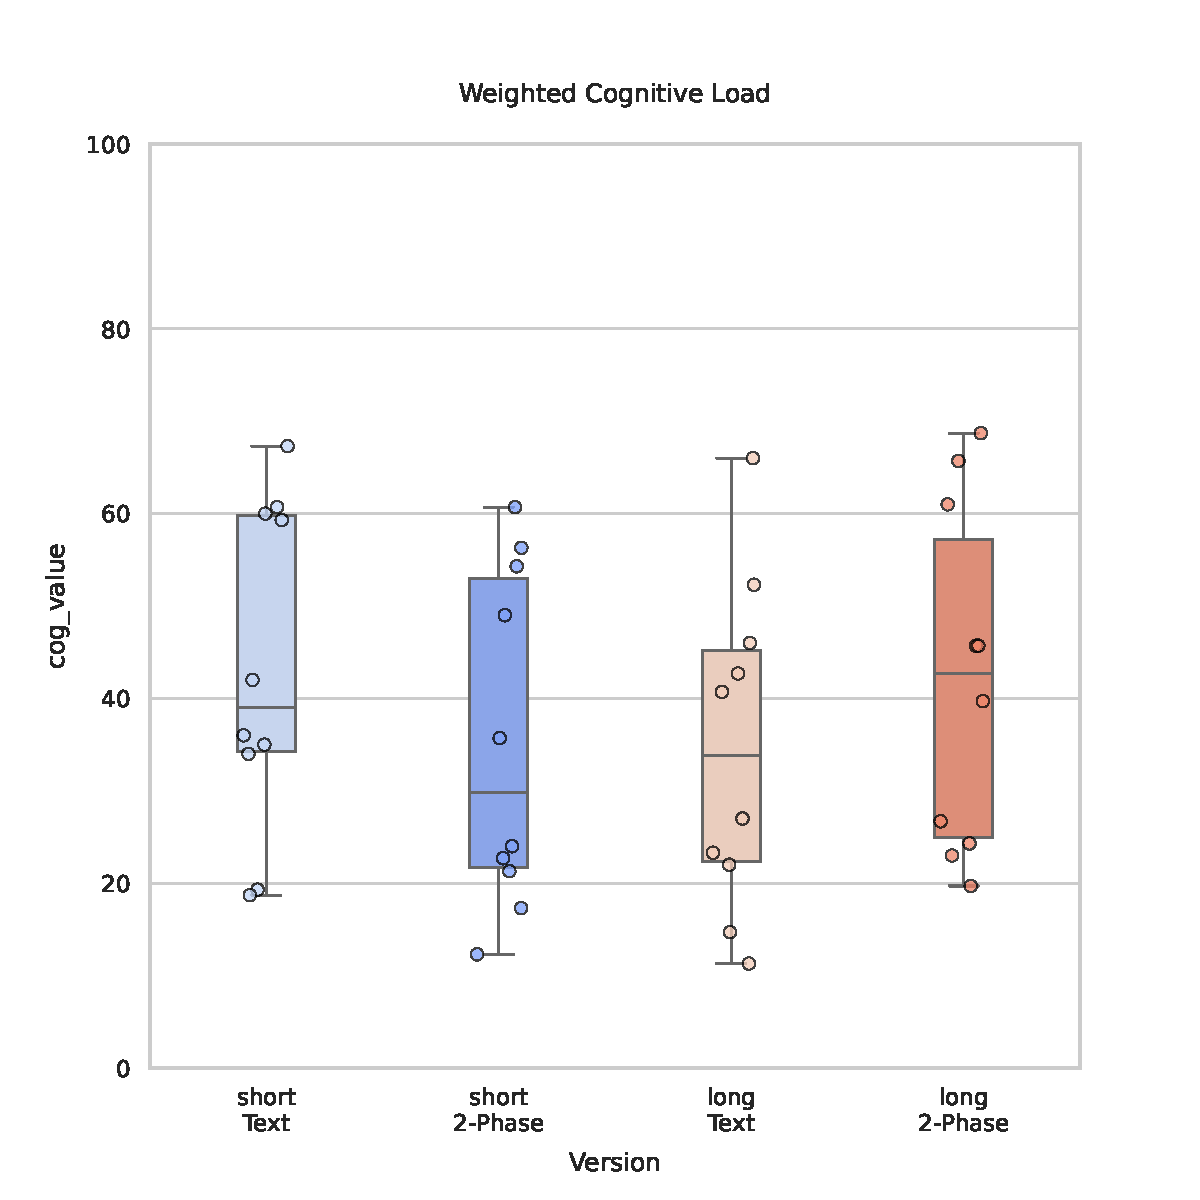
\includegraphics[width=0.95\textwidth]{content/image/results/nasatlx_final_value.pdf}
            }
            \caption{NASA-TLX Weight Score: The Long Two-Phase Interface exhibits the highest weighted cognitive load with a median of $42.70$, a mean of $42.02$. This is higher than the long text interface, which has a median cognitive load of $33.85$ and a mean of $34.60$. However, the short text interface demonstrates a higher cognitive load with a median of $39.00$, a mean of $43.23$, compared to the short two-phase interface, which has a median of $29.85$, a mean of $35.36$. The standard deviation is similar across groups at around $18$.}
            \Description{A box plot comparing weighted cognitive load scores across four interface conditions: short text, short two-phase, long text, and long two-phase. The y-axis is labeled "Weighted Cognitive Load" and ranges from 0 to 100. Each condition is represented by a box with whiskers, and individual data points are plotted as circles. The short text and long two-phase interfaces show higher cognitive load distributions, while the short two-phase and long text interfaces show lower distributions. The title reads "Weighted Cognitive Load."}
            \label{fig:nasatlx-final1}
        \end{subfigure}
    }
    \hfill
    \adjustbox{valign=t}{ % Adjust second subfigure for top alignment
        \begin{subfigure}{0.49\textwidth}
            \centering
            \adjustbox{valign=t}{
                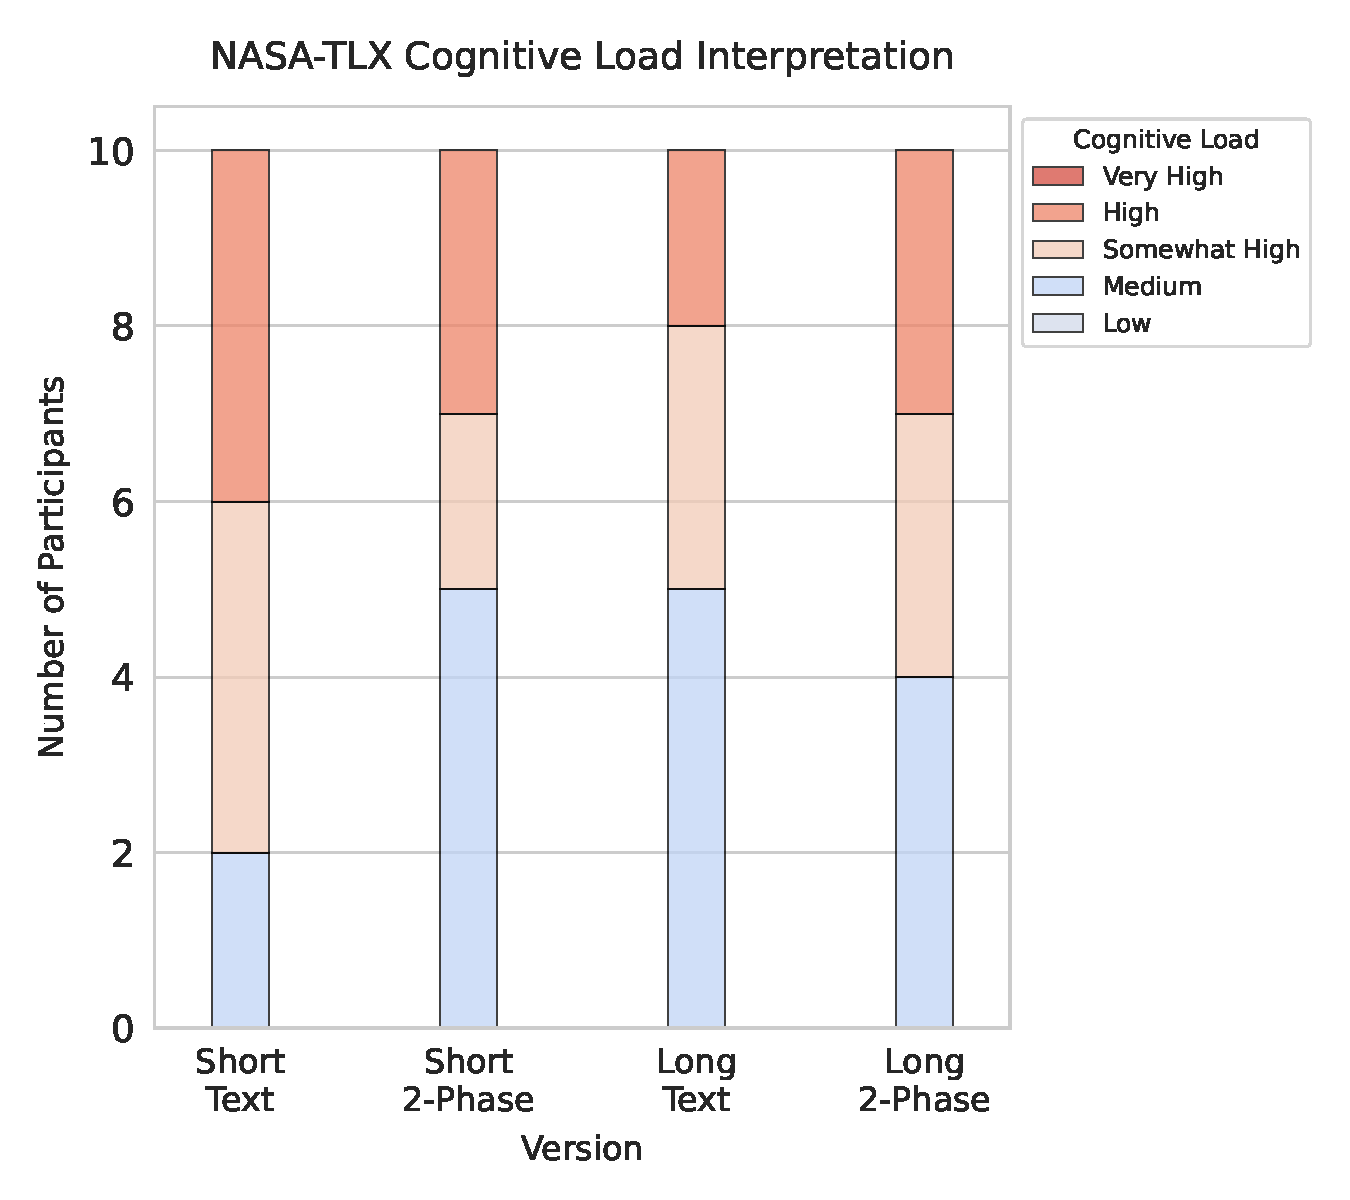
\includegraphics[width=1.05\textwidth]{content/image/results/nasatlx_cog_value_interpreted.pdf}
            }
            \caption{NASA-TLX Cognitive Interpretation: More participants in the short text interface, totaling $8$, reported a somewhat high or above cognitive load, which is significantly higher compared to the $5$ participants who reported similarly for the short two-phase interface. However, the long two-phase interface saw slightly more participants, $6$ in total, reporting somewhat high or above cognitive load compared to the long text interface.}
            \Description{Stacked bar chart showing the number of participants experiencing different levels of cognitive load across four interface versions: Short Text, Short 2-Phase, Long Text, and Long 2-Phase. The y-axis represents the number of participants (from 0 to 10), and the legend differentiates five cognitive load levels: Low, Medium, Somewhat High, High, and Very High. The chart highlights more participants reporting higher cognitive loads for short text-based interfaces.}
            \label{fig:nasatlx-final2}
        \end{subfigure}
    }
    \caption{This figure shows the box plot results for weighted NASA-TLX scores across experiment groups and participant counts based on individual score interpretations. In~\ref{fig:nasatlx-final1}, we observe a downward trend in cognitive load for the short QS, while the long QS shows an upward trend. Interestingly, there is a counterintuitive downward trend between short and long text interfaces. In~\ref{fig:nasatlx-final2}, these trends are clearer when NASA-TLX scores are grouped into five tiers.}
    \Description{Two figure side by side, a box plot to the left and a stacked bar chart to the right, representing the weighted NASA-TLX distributions and the interpretations respectively.}
    \label{fig:nasatlx-final}
\end{figure}

\subsection{Overall Cognitive Load}
\label{sec:cog}
Weighted NASA-TLX uses a continuous $0$-$100$ score, with higher values denoting greater cognitive load. We use predefined mappings of NASA-TLX scores to cognitive levels: low, medium, somewhat high, high, and very high, as described by~\textcite{hart1988development}. Results are shown in Figure~\ref{fig:nasatlx-final}, with value interpretations presented in Figure~\ref{fig:nasatlx-final2}.

We design a hierarchical ordinal regression Bayesian model that estimates a linear predictor incorporating length, interface, and their interaction effect, accounting for the data's sparsity. The interaction terms are modeled using an LKJ prior to regularize the correlations between length and interface levels. We present details of the model in Appendix XX.

While results (Figure X) are not statistically significant in Bayesian terms, as 0 does not lie outside the high-density interval, the interval reflects the 94\% probability that the true parameter lies within it. This provides quantifiable evidence of trends while transparently accounting for uncertainties:
\begin{itemize}
    \item Increased option length trends to reduced cognitive load with a posterior probability of approximately $69.4\%$, corresponding to a medium-to-large effect size ($d = 0.61$). This reflects a median cognitive load of $33.85$ (mean = $34.60$, SD = $17.69$) compared to a median of $39.00$ (mean = $43.23$, SD = $17.65$).
    \item Within short QS, the interactive interface trends to reduced cognitive load, with a posterior probability of $64.5\%$ supporting the reduction and a small-to-medium effect size ($d = 0.49$). Participants report a median cognitive load of $29.85$ (mean = $35.36$, SD = $18.17$) under the two-phase interface compared to a median of $39.00$ (mean = $43.23$, SD = $17.65$) under the text interface.
    \item For the long QS, there trends a small increase in cognitive load with a posterior probability of $61.7\%$ and a small effect size ($d = 0.18$). The median cognitive load is $42.70$ (mean = $42.02$, SD = $18.48$) under the two-phase interface compared to $33.85$ (mean = $34.60$, SD = $17.69$) in the text interface.
\end{itemize}

This result contradicts our hypothesis that more options would increase cognitive load and that interfaces can reduce it. Thus, we explore qualitative results to identify possible explanations. To understand the similarities and differences in sources of cognitive load (\textbf{RQ2b}), we analyze qualitative results across the six NASA-TLX subscales: mental demand, physical demand, temporal demand, effort, frustration, and performance. Detailed analyses are provided in Appendix XX.

\subsection{Common Sources of Cognitive Load}
Our analysis reveals several themes across different cognitive load subscales. We identify four themes common to all experimental conditions.

\textbf{Preference Construction} is cited by 97.5\% (N=39) of participants as a significant source of mental demand, consistent with prior literature suggesting that preferences are often constructed in context rather than fixed~\cite{lichtensteinConstructionPreference2006}. Specific tasks contributing to this demand include evaluating the relative importance between options (e.g.,\smallquote{S002}{Figuring out\bracketellipsis how much I prioritize option 1 over option 2}, 40\% ($N=16$)), making trade-offs due to limited resources (e.g.,\smallquote{S005}{\bracketellipsis very hard to take decisions~\ldots I felt that multiple options deserve equal amounts of credit~\ldots but you have given very limited credit.}, 42.5\% ($N=17$)), and deciding the exact number of votes (e.g.,\smallquote{S023}{\bracketellipsis having to pick how many upvotes would go to each one}, 70\% ($N=30$)).

\textbf{Budget Management} emerges as a source of both mental and temporal demand. 25\% (N=10) of participants describe the challenge of working with limited credits while trying to maximize their allocation (e.g.,~\smallquote{S032}{~\bracketellipsis for certain societal issues, you had to~\ldots take away from other issues you could support}). An equal percentage of participants find it mentally taxing to keep track of remaining credits (e.g.,~\smallquote{S006}{~\bracketellipsis looking at the remaining credits, I'm trying to mentally divide that up before I start allocating}).

\textbf{Operational Actions} refer to reactive efforts addressing immediate, tactical needs. These actions involve direct task execution, responding to constraints without reflection on broader, long-term implications. Examples include adjusting choices to stay within budget (e.g.,~\smallquote{S003}{I had to alter~\bracketellipsis I kept going under budget}), re-reading options (e.g.,~\smallquote{S010}{I just had to reread it again}), completing questions efficiently (e.g.,~\smallquote{S010}{I was trying to be efficient in responding to the question}), and interacting with the survey interface (e.g.,~\smallquote{S023}{I was trying to be efficient in responding to the question}). 40\% (N=16) of participants attribute Operational actions to temporal demand. Additionally, 37.5\% (N=15) attribute this cause to frustration, and 32.5\% (N=13) attribute it to performance. While this is a commonly cited source across experiment conditions, there are different distributions. 

\textbf{Internal Conflicts and Regretful Trade-offs} are cited by 27.5\% (N=11) of participants as a source of frustration, particularly when making decisions that conflict with personal values or societal preferences. These findings suggest the potential benefits of Quadratic Surveys (QS) in encouraging participants to balance broader societal considerations and the broader population with their personal preferences.

\begin{displayquote}
I would have loved to have given more to other groups~\ldots and I felt stressed~\bracketellipsis it's a group that you know is still~\ldots you know~\ldots important~\bracketellipsis
\noindent \hfill -- S020, long text interface
\end{displayquote}

% \textbf{Social Responsibility} was considered by 20\% of participants (N=8) regarding performance. They wonder how their final vote counts would be perceived by others~(\smallquote{S041}{I don't want people to think that I just like don't care about <ethnicity> people at all}) or influence real-world decision-making~(\smallquote{S027}{Some of these things might \ldots have outcomes that I didn't foresee}).

\subsection{Different Sources of Cognitive Load}
There are several notable differences between the text and two-phase interfaces. 

First, regardless of length, when analyzing performance, which refers to a person's perception of their success in completing a task, participants describe their performances differently. We categorize them into indications of satisficing behaviors(``good enough''), exhausting their effort (i.e., ``done their best,''), or feeling positive (i.e., ``feeling good.'') There are twice as many participants using the two-phase interface to report a positive feeling about their final submission~(55\% v.s 30\% (N=11 vs. 6)).

Second, 70\% (N=14) of text interface participants attribute operational actions as contributors to effort, double the percentage observed in the two-phase interface group (35\%, N=7). This partially echoes the finding that 90\% (N=18) of text interface participants report mental demand from deciding the exact number of votes, compared to 60\% (N=12) in the two-phase interface group.

% 30\% (N=6) Participants from the long survey attribute many option as source of mental demand compared to none from the short survey.

The distinction between the text and two-phase interfaces becomes more pronounced in the context of the long survey. 80\% of the long text interface participants (N=8) attribute operational actions to effort, compared to only 20\% (N=2) in the long two-phase interfaces. Conversely, 90\% of long two-phase interface participants (N=8) attribute effort to strategic actions, compared to 50\% (N=5) in the text interface. \textbf{Strategic operations} refer to reflective decisions oriented toward long-term goals. They focus on determining priorities, considering broader implications, and aligning actions with overarching objectives. Mental demand shows similar patterns. 80\% of participants~($N=8$) in the long text interface focused on a narrower scope, emphasizing personal relevance and comparing fewer options. In contrast, 90\% of participants ($N=9$) in the long two-phase interface consider broader societal impacts and evaluate more options simultaneously, compared to 30\% ($N=3$) in the text interface. The following quotes highlight these differences:

\begin{displayquote}
Trying to figure out what upvotes I should give~\bracketellipsis went back and forth between those two. \bracketellipsis it was very mentally tasking for me. \hfill\quoteby{S015~(LT)}
\end{displayquote}

\begin{displayquote}
\bracketellipsis really having to think, especially with so many different societal issues. How do I personally prioritize them? And to what extent do I prioritize them? \hfill\quoteby{S009~(LI)}
\end{displayquote}

These qualitative differences highlight the variation in~\textbf{levels of engagement} with the survey content. Participants using the two-phase interface report higher satisfaction qualitatively about their performance. For the long survey, they considered broader aspects across different options and how to strategically allocate their credits. 



%  moved to time analysis
% Third, when comparing the text and two-phase interfaces in short surveys, 50\% of participants (N=5) express concerns about the time spent on decision-making, reporting that they invest more time and effort than expected, prompting them to rush. However, the two-phase interface reduced this, with only one participant in the short survey group reporting similar concerns.

